\begin{savequote}[75mm]
The feeling is less like an ending than just another starting point.
\qauthor{Chuck Palahniuk}
\end{savequote}

\chapter{Combined Run 1 $H\rightarrow WW^{*}\rightarrow \ell\nu\ell\nu$ results}

\section{Introduction}

In the final statistical analysis of \HWWfull, the dedicated gluon-gluon fusion and vector boson fusion sensitive signal regions are all combined into a single fit to determine the main parameters of interest, the Higgs signal strength $\mu$ and mass $m_H$. Therefore, while the specific requirements applied for the VBF sensitive analysis are discussed in chapter 5, the final measurement of these parameters can only be discussed in combination with the results of the ggF dedicated analysis. For example, because ggF Higgs production is considered a background in the VBF analysis, the ggF dedicated signal regions can actually constrain the normalization of this background in the VBF dedicated region.

This chapter presents the combined interpretation of results in the \HWWfull analysis for gluon fusion and vector boson fusion Higgs production. First, the results of the dedicated gluon fusion search are presented. Then, a comparison of the individual production mode signal strengths ($\mu_{\ggF}$ and $\mu_{\VBF}$ and a measurement of the combined signal strength ($\mu$) are shown. Subsequently, the measured values of the Higgs couplings to fermions and vector bosons is presented. Finally, the cross section measurement for ggF and VBF production are shown. 

\section{Results of dedication gluon fusion \HWWfull search}

The details of the dedicated gluon fusion \HWWfull search are not discussed in this thesis and instead left to more comprehensive sources\cite{WW2015}. However, a brief summary of the results are essential for describing the results of the full analysis and interpreting the results of the dedicated VBF search in this broader context. 

Table~\ref{tab:fitregions} shows the individual signal regions that were input into the final statistical fit. The ggF dedicated bins use $\mTH$ as their discriminating variable and are separated into bins of $\pT$ of the subleading lepton as well. The VBF dedicated bin uses the $\bdt$ distribution as its final discriminant. 

\begin{table*}[tb!]
\centering%
\captionsetup{justification=centering}

%--------------------------------------------------------------------------------
\begin{tabular*}{\textwidth}{
  p{0.3\textwidth}
  l %p{0.100\textwidth}
  l %p{0.100\textwidth}
  l
  c
  c
}
\\
\dbline
\multicolumn{4}{c}{SR category $i$}
&
&\multicolumn{1}{l}{\multirow{2}{*}{Fit var.}}
\\
\clineskip%
\cline{1-4}%
\clineskip%
$\Njet$, flavor
&${\otimes\,}\mll$
&${\otimes\,}\pTsublead$
&${\otimes\,}\ell_2$
&
&
\\
\sgline
$\NjetEQzero$ \\
\quad $\DFchan$     &${\otimes\,}[10,30,55]$ &${\otimes\,}[10,15,20,\infty]$ &${\otimes\,}[e,\mu]$ &&$\mTH$ \\
\quad $\SFchan$     &${\otimes\,}[12,55]$    &${\otimes\,}[10,\infty]$       &                     &&$\mTH$ \\
\sgline
$\NjetEQone$ \\
\quad $\DFchan$     &${\otimes\,}[10,30,55]$ &${\otimes\,}[10,15,20,\infty]$ &${\otimes\,}[e,\mu]$ &&$\mTH$ \\
\quad $\SFchan$     &${\otimes\,}[12,55]$    &${\otimes\,}[10,\infty]$       &                     &&$\mTH$ \\
\sgline
$\NjetGEtwo$ ggF \\
\quad $\DFchan$     &${\otimes\,}[10,55]$    &${\otimes\,}[10,\infty]$       &                     &&$\mTH$ \\
\sgline
\multicolumn{2}{l}{$\NjetGEtwo$ VBF} \\
\quad $\DFchan$     &${\otimes\,}[10,50]$    &${\otimes\,}[10,\infty]$       &                     &&$\bdt$ \\
\quad $\SFchan$     &${\otimes\,}[12,50]$    &${\otimes\,}[10,\infty]$       &                     &&$\bdt$ \\
\end{tabular*}
\caption{
  All signal regions definitions input into final statistical fit\cite{WW2015}.
}
\label{tab:fitregions}
\end{table*}
%eof

Table~\ref{tab:final-yields} shows the yields in the various signal regions in both data and expected signal and backgrounds. The yields for signal and background are all scaled according to the final normalizations calculated in the fit. 


\begin{table}[h!]
\centering
\captionsetup{justification=centering}

%\begin{tabular*}{0.480\textwidth}{p{0.075\textwidth} p{0.180\textwidth} l}
\hspace{-10pt}
\begin{tabular}{|c|c|c|c|c|}
\hline
 & $N_{\rm obs}$ & $N_{\rm bkg}$ & $N_{\rm ggF}$ & $N_{\rm VBF}$ \\ \hline
$\Njet = 0$ & $3750$ & $3430 \pm 90$ & $300 \pm 50$ & $8 \pm 4$ \\ \hline
$\Njet = 1$ & $1596$ & $1470 \pm 40$ & $102 \pm 26$ & $17 \pm 5$ \\ \hline
$\Njet \geq 2$, $\rm ggF$ $e\mu$ & $1017$ & $960 \pm 40$ & $37 \pm 11$ & $13 \pm 1.4$ \\ \hline
$\Njet \geq 2$, $\rm VBF$ & $130$ & $99 \pm 9$ & $7.7 \pm 2.6$ & $21 \pm 3$ \\ \hline
\end{tabular}

\caption{
Post-fit yields in the different ggF and VBF dedicated signal regions\cite{WW2015}. 
}
\label{tab:final-yields}
\end{table}

Figure~\ref{fig:ggF-mT} shows the final post-fit $\mTH$ distribution in the $\Njet \leq 1$ regions. The data are very consistent with the hypothesis of ggF Higgs production. 

\begin{figure}[h!]
  %\vspace{20pt}
  \centering
  \captionsetup{justification=centering}

  %\hspace*{-32pt}
  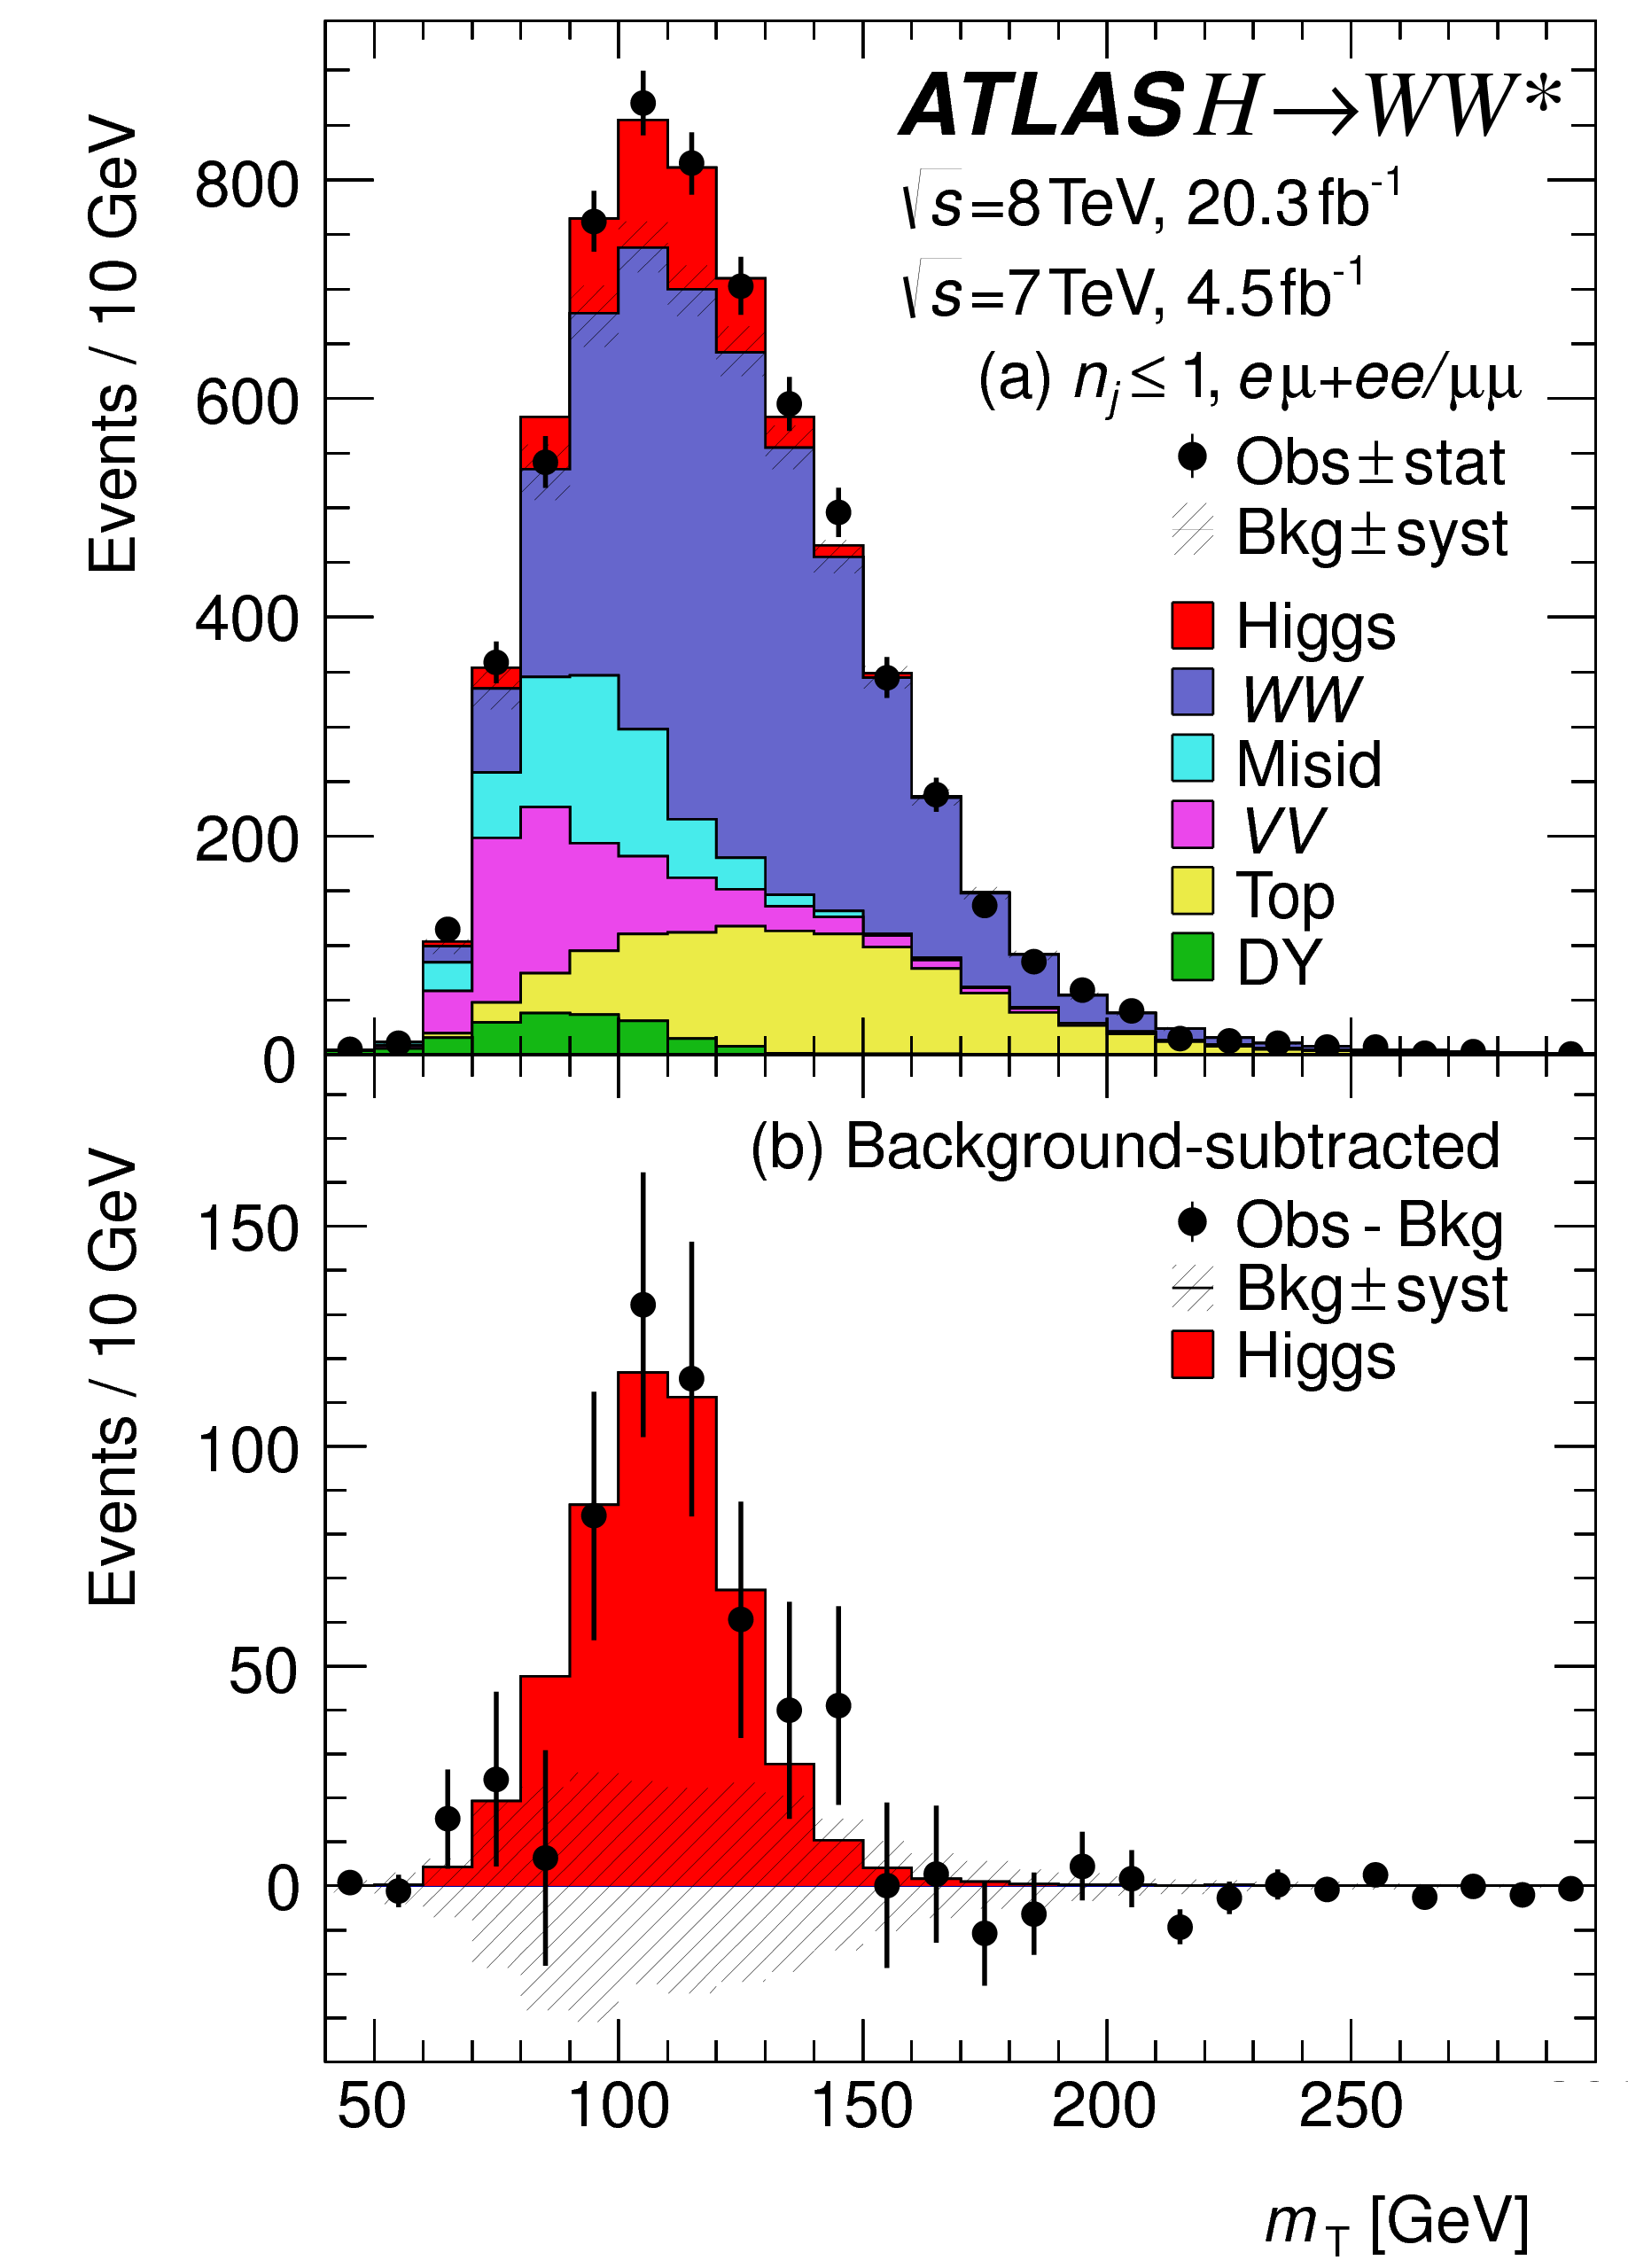
\includegraphics[width=0.6\textwidth]{figures/ggF_mT}
  \caption{Post-fit $\mTH$ distribution in the $\Njet \leq 1$ regions\cite{WW2015}.}
  \label{fig:ggF-mT}
\end{figure}

These yields are used as input, along with the VBF results in chapter 5, for the physical interpretation of results presented in subsequent sections. 

\section{Signal strength measurements in ggF and VBF production}

When all of the signal regions are combined in the fit, there can be a combined measurement of the signal strength as well as the individual ggF and VBF signal strengths. The combined signal strength is the ratio of the sum of the gluon fusion and VBF cross sections to the theory prediction, or a singal strength for the total Higgs production cross section that this analysis is sensitive to. The final measured combined signal strength $\mu$ is measured shown in equation~\ref{eqn:final-mu}.

\begin{equation}
\begin{array}{llllll}
 \mu
 &= 1.09%
 &^{+0.16}_{-0.15}\,(\textrm{stat.})%
 &^{+0.08}_{-0.07}\,\Big(\!\begin{tabular}{c}{\rm\footnotesize expt}\\ \noalign{\vskip -0.50truecm}{\rm\footnotesize syst}\end{tabular}\!\Big)%
 &^{+0.15}_{-0.12}\,\Big(\!\begin{tabular}{c}{\rm\footnotesize theo}\\ \noalign{\vskip -0.50truecm}{\rm\footnotesize syst}\end{tabular}\!\Big)%
 &{\PM}0.03\,\Big(\!\begin{tabular}{c}{\rm\footnotesize lumi}\\ \noalign{\vskip -0.50truecm}{\rm\footnotesize syst}\end{tabular}\!\Big)%
 \\
 \clineskip
 &= 1.09 &^{+0.16}_{-0.15}\,\textrm{(stat)} &^{+0.17}_{-0.14}\,\textrm{(syst)}
 \\
 \clineskip
 \clineskip
 &= 1.09 &^{+0.23}_{-0.21}.
\end{array}
\label{eqn:final-mu}
\end{equation}

Figure~\ref{fig:mu-val} gives the best fit signal strength $\hat{\mu}$ as a function of hte hypothesized Higgs mass. The value at 125.36 \GeV corresponds to the $\mu$ quoted in equation~\ref{eqn:final-mu}. This value of the Higgs mass is used because it is the most precise mass measurement from ATLAS, a result of the combined $\gamma\gamma$ and $ZZ$ mass measurements\cite{MassMeasurement}.

\begin{figure}[h!]
  %\vspace{20pt}
  \centering
  \captionsetup{justification=centering}

  %\hspace*{-32pt}
  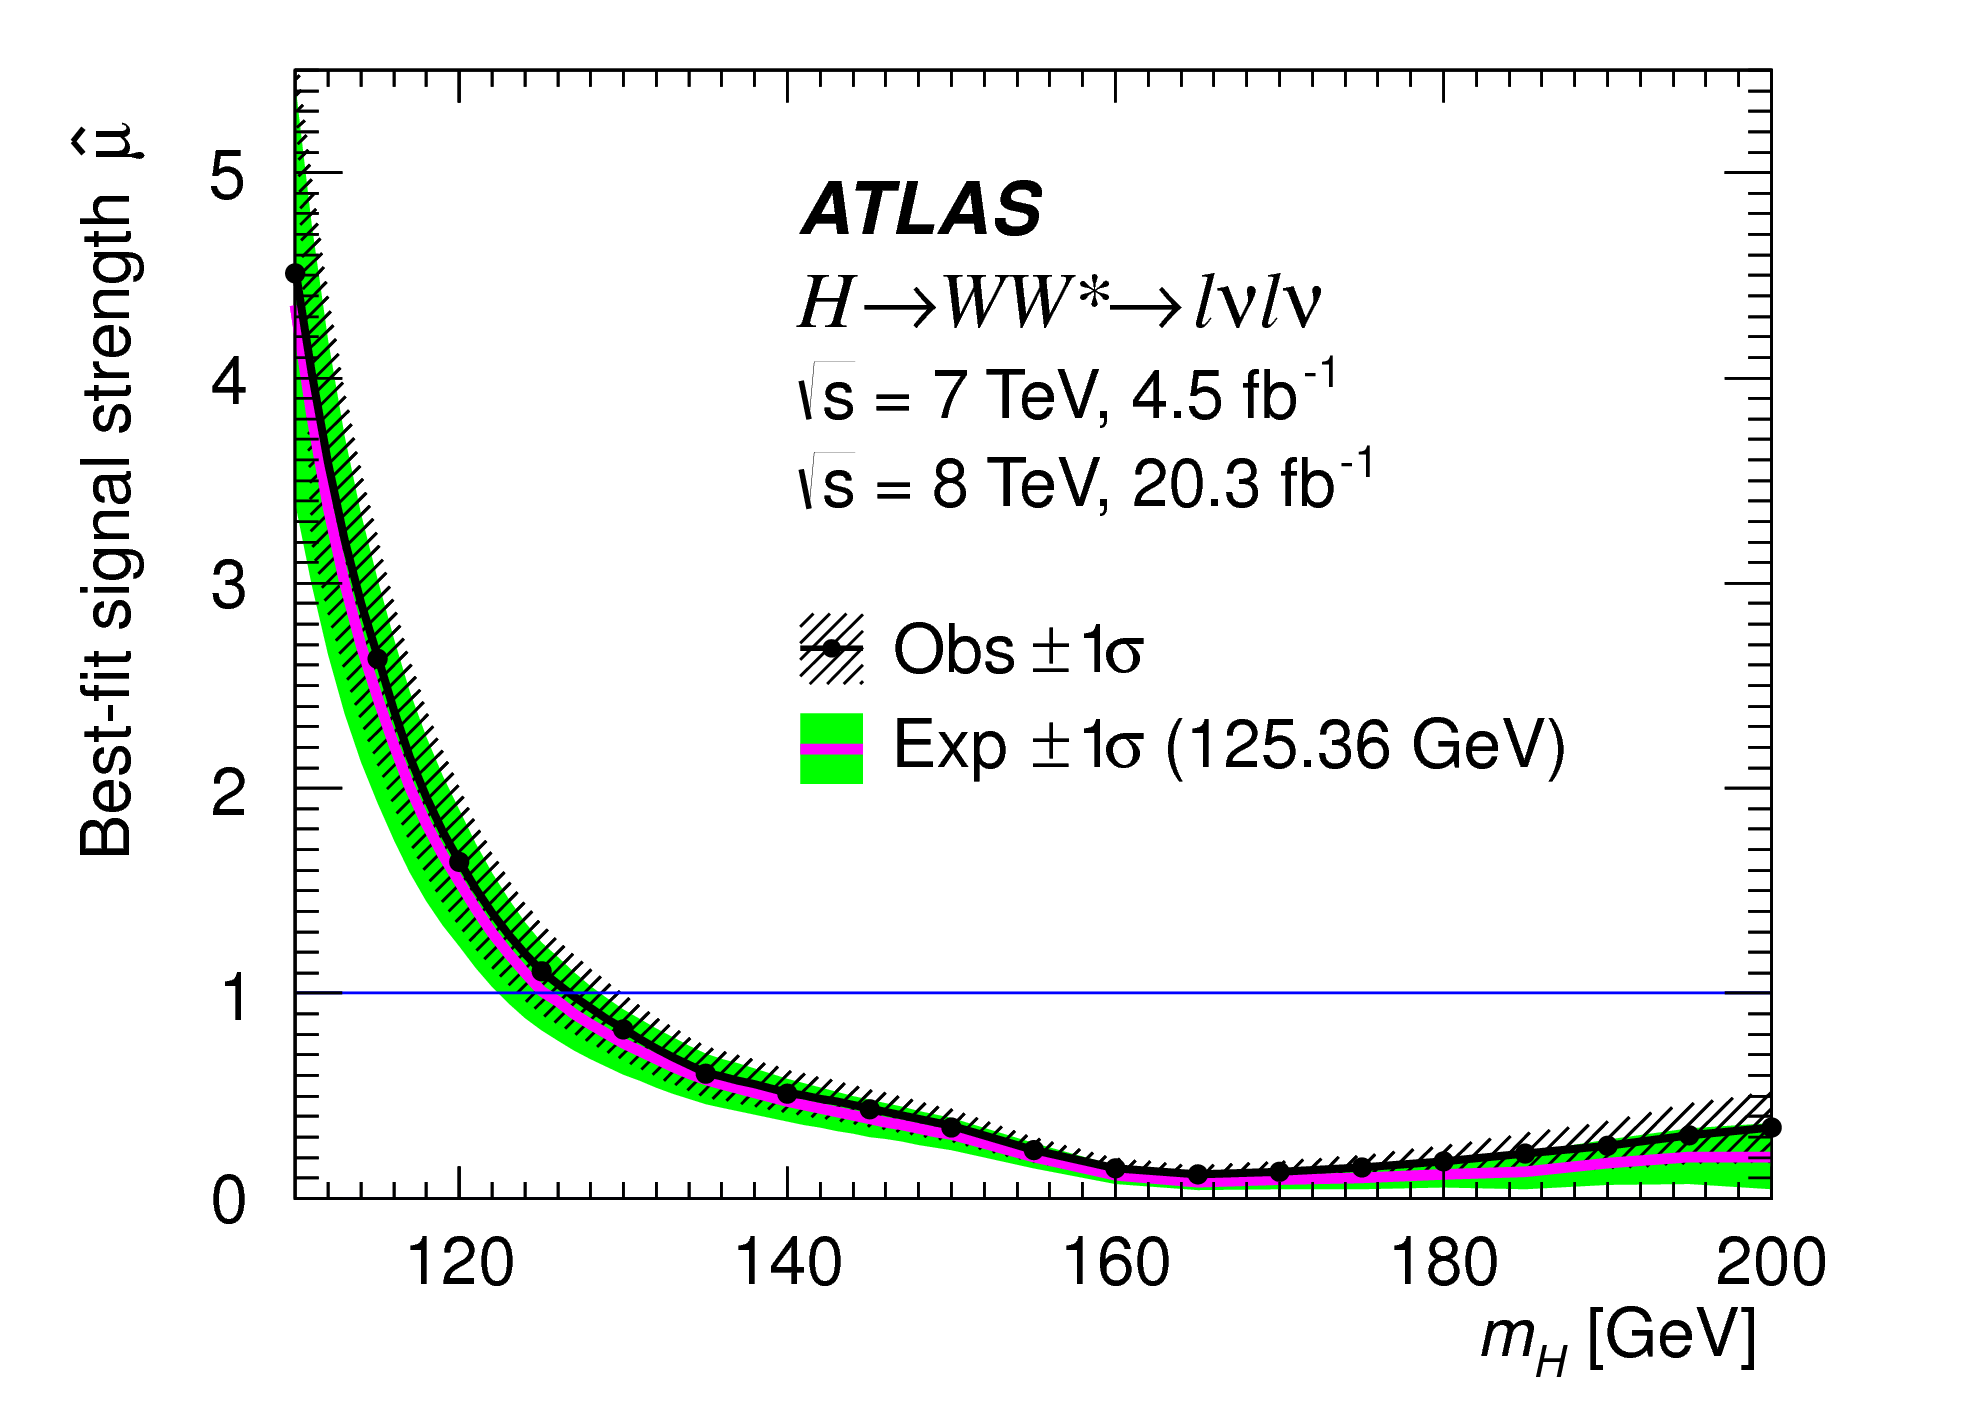
\includegraphics[width=0.8\textwidth]{figures/mu_mass}
  \caption{Best fit signal strength $\hat{\mu}$ as a function of hypothesized $m_{H}$\cite{WW2015}.}
  \label{fig:mu-val}
\end{figure}

As explained in chapter 3, a probability $p_0$ can be computed using the test statistic $q_0$ to quantify the probability that the background could fluctuate to produce an excess at least as large as the one observed in the data. The local $p_0$ value is shown in figure~\ref{fig:p0} as a function of $m_H$. The minimum $p_0$ value is at $m_H = 130 \GeV$ and coresponds to a significance of $6.1\sigma$. The curve is relatively flat and the significance is the same at 125.36 \GeV within the quoted precision. The expected significance for a signal with strength $\mu = 1.0$ is $5.8\sigma$. This represents the first discovery level significance measurement in the \HWWfull analysis. 

\begin{figure}[h!]
  %\vspace{20pt}
  \centering
  \captionsetup{justification=centering}

  %\hspace*{-32pt}
  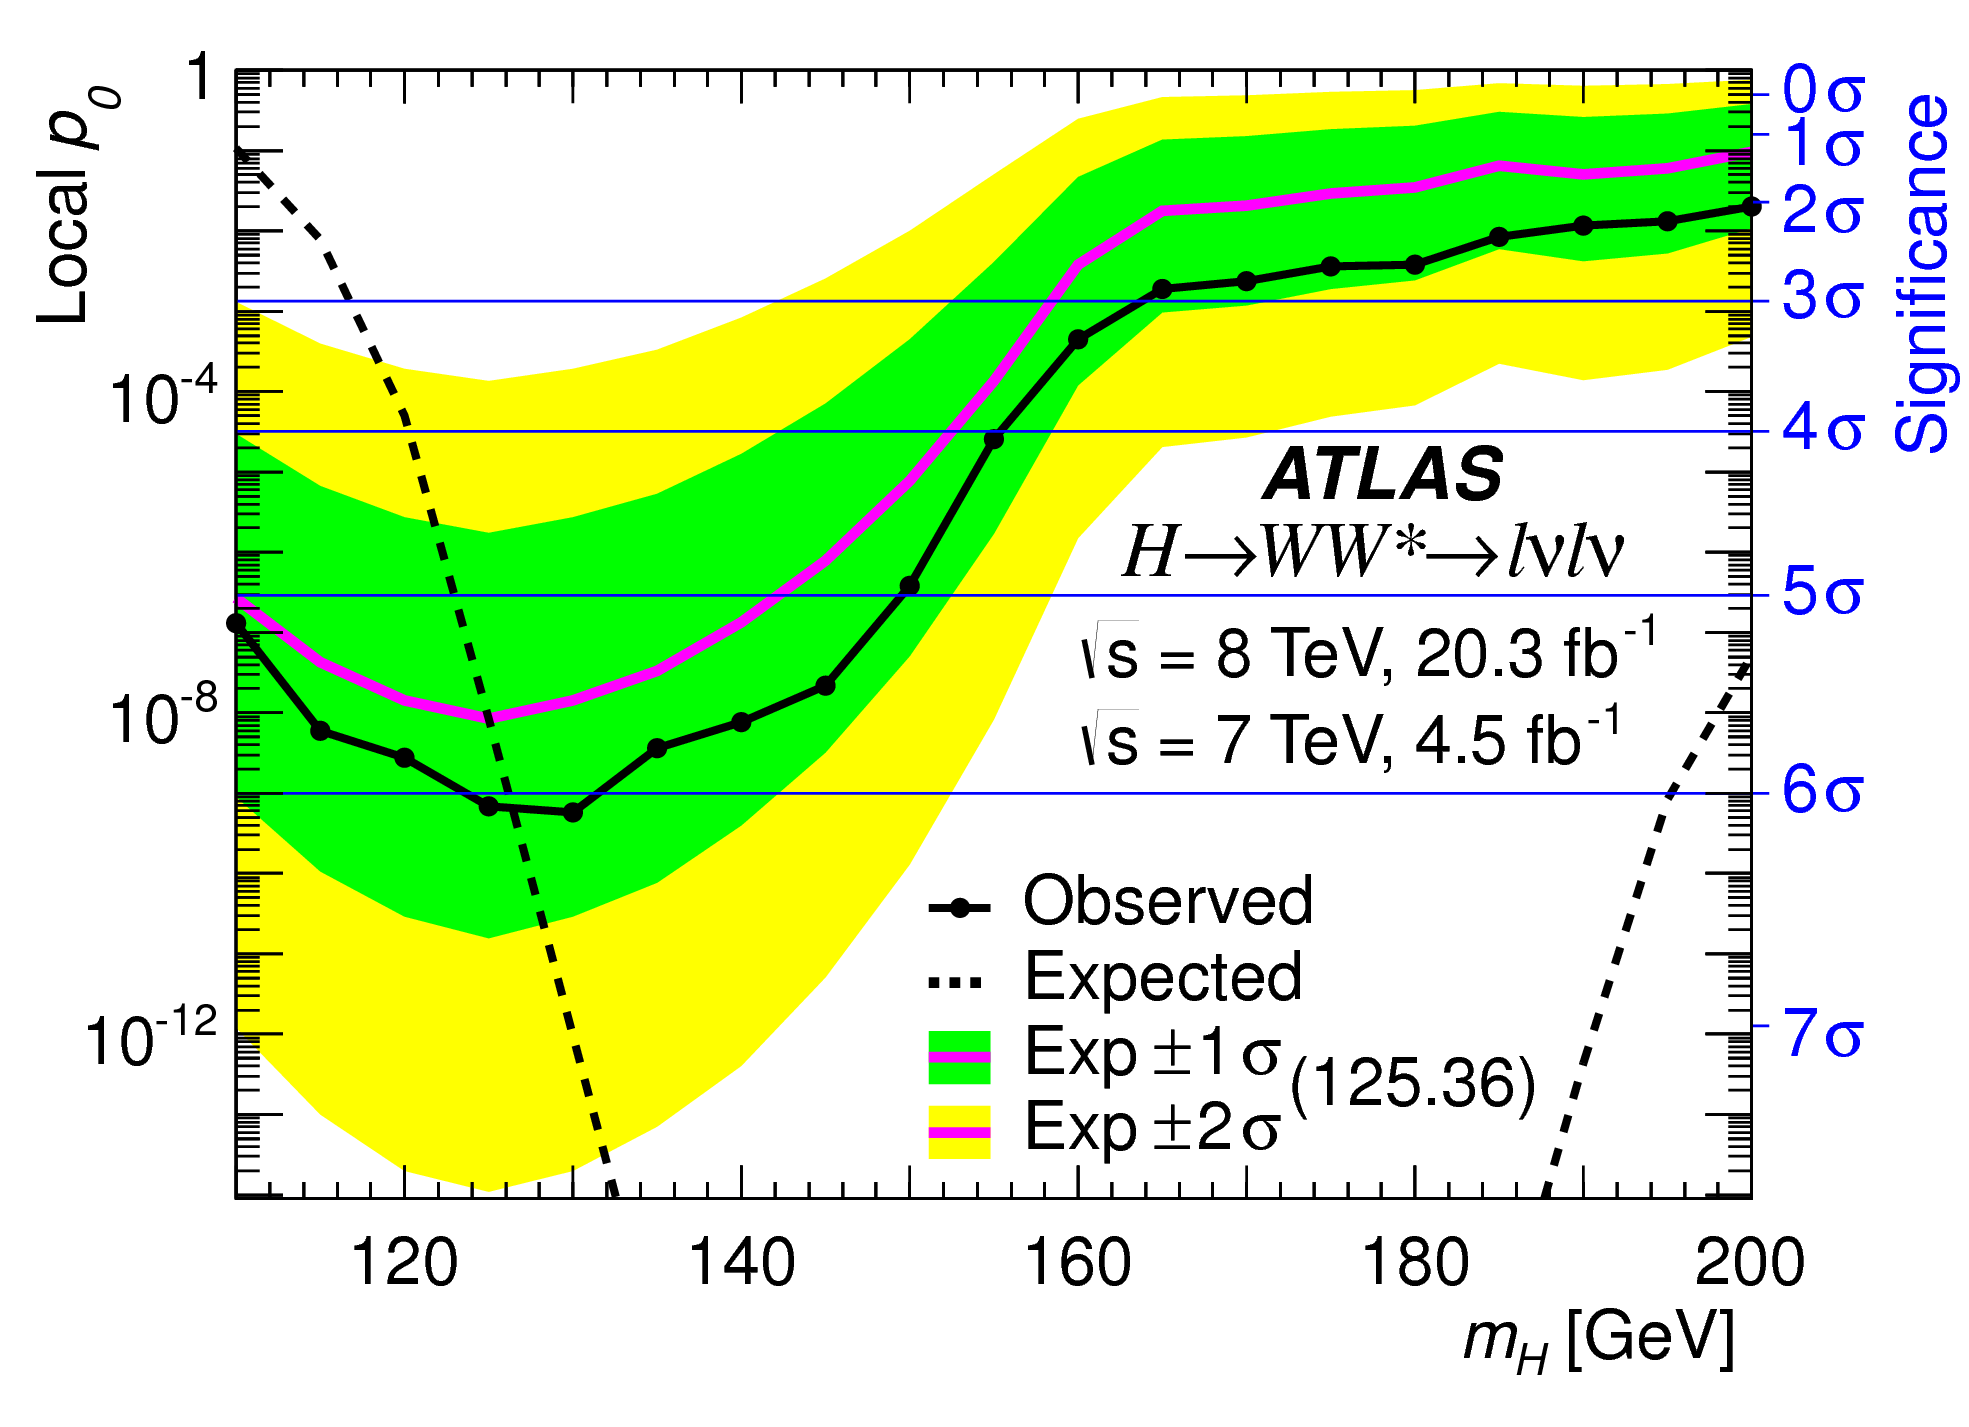
\includegraphics[width=0.8\textwidth]{figures/WW_p0}
  \caption{Local $p_0$ as a function of $m_H$\cite{WW2015}.}
  \label{fig:p0}
\end{figure}

All the results presented so far in this section have been for the combined gluon fusion and VBF production modes. However, each signal strength can be calculated separately in the likelihood as well. There are two ways to do this. First, the likelihood can be parameterized in terms of a single parameter, the ratio of the VBF and gluon fusion signal strengths. With this method, the significance of the VBF observation can be evaluated. Figure~\ref{fig:mu_ratio} shows the likelihood as a function of the ratio $\mu_{\VBF}/\mu_{\ggF}$.

\begin{figure}[h!]
  %\vspace{20pt}
  \centering
  \captionsetup{justification=centering}

  %\hspace*{-32pt}
  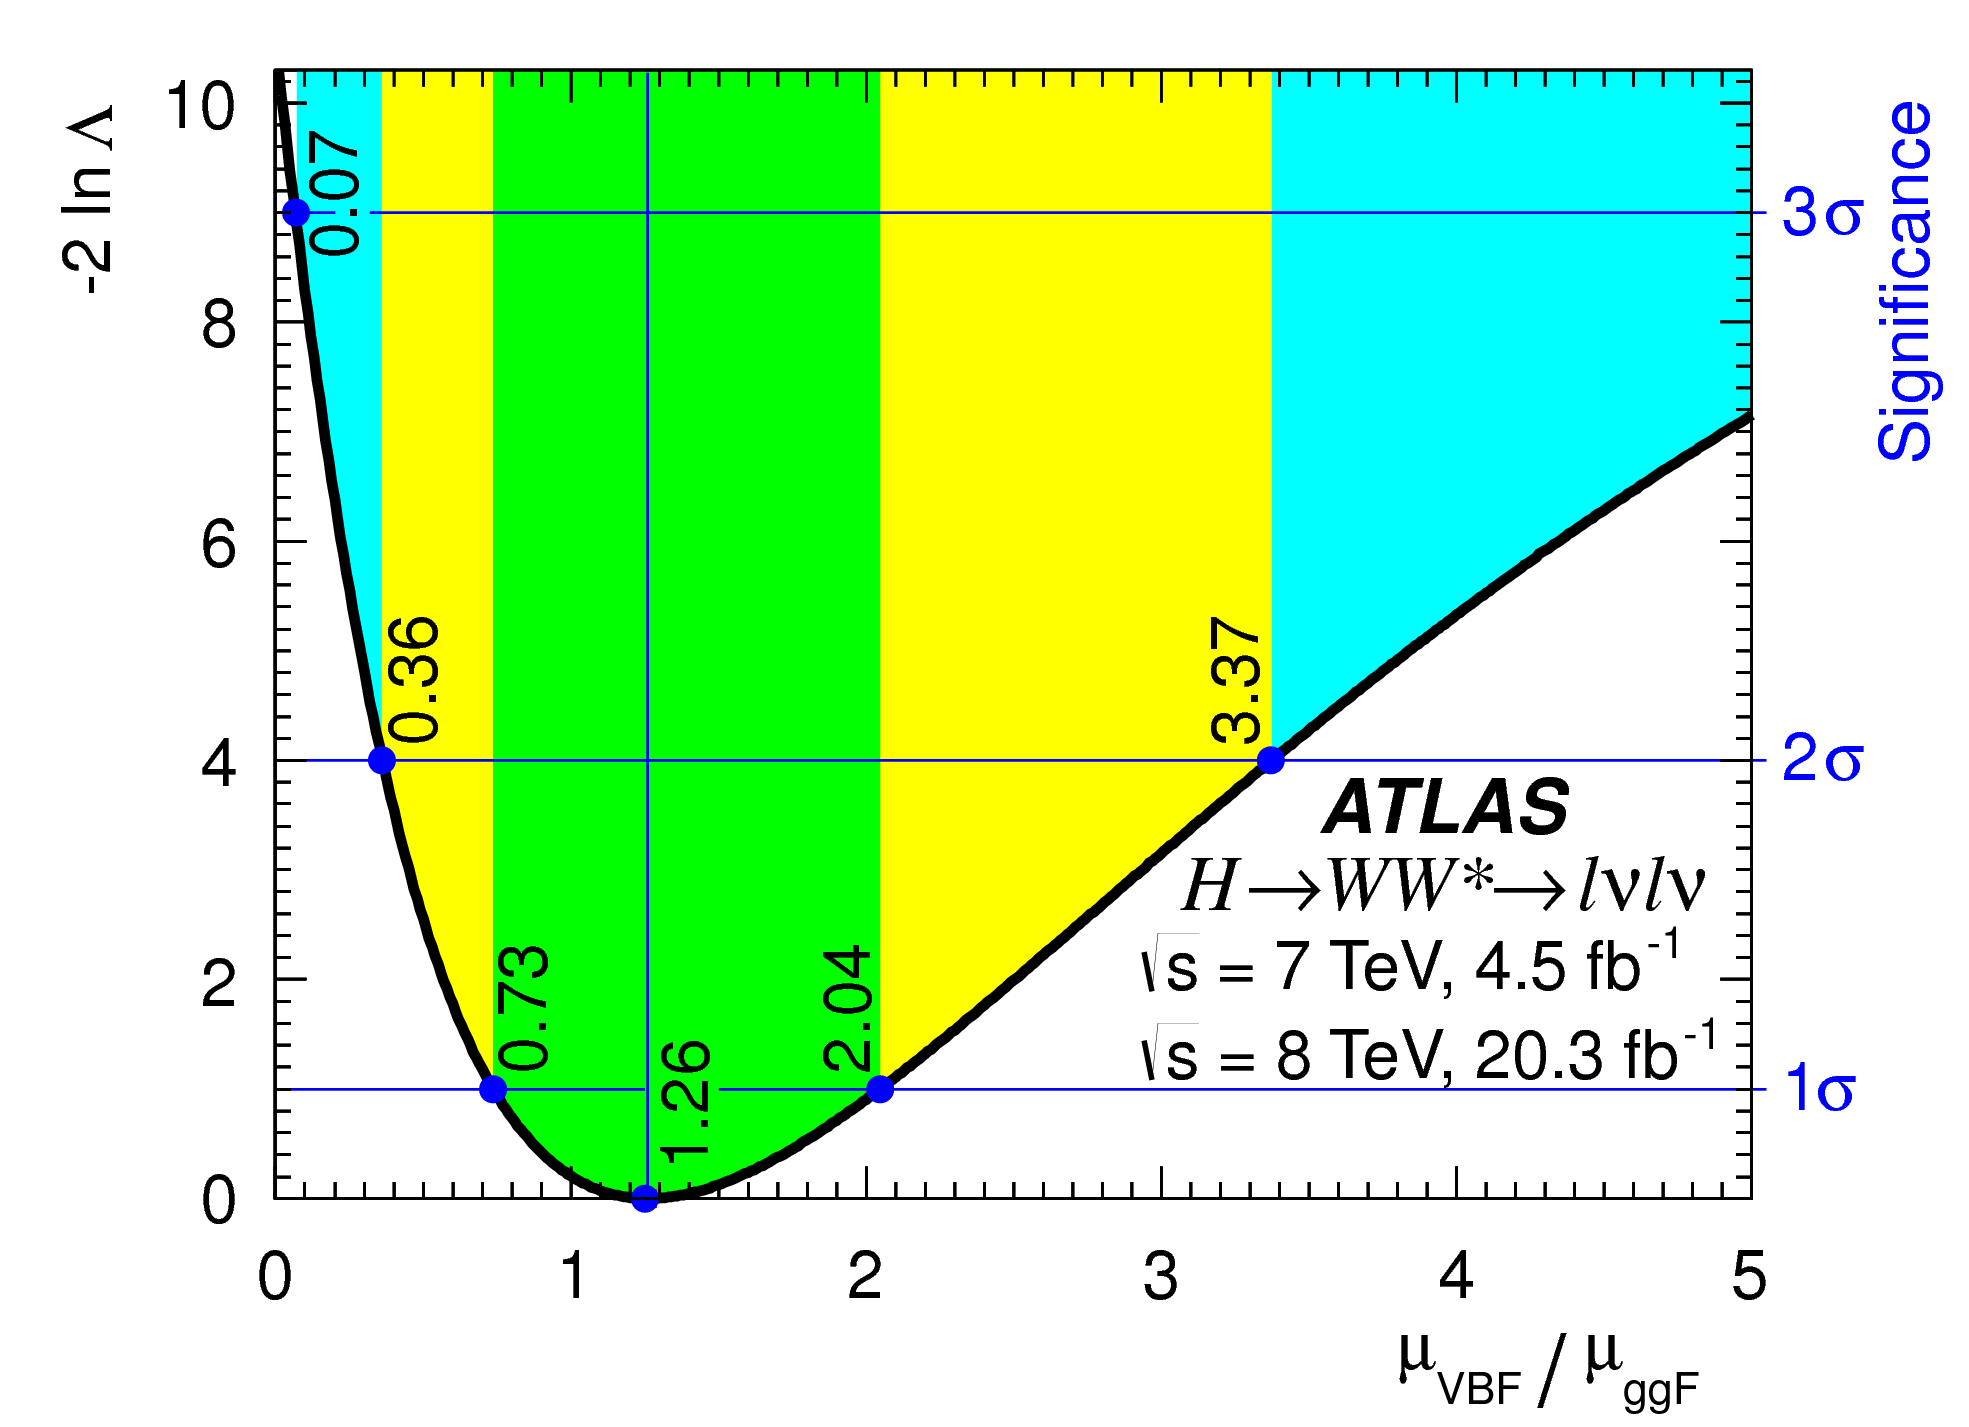
\includegraphics[width=0.8\textwidth]{figures/WW_muratio}
  \caption{Likelihood as a function of $\mu_{\VBF}/\mu_{\ggF}$\cite{WW2015}.}
  \label{fig:mu_ratio}
\end{figure}

The best fit value of the ratio of signal strengths is shown in equation~\ref{eqn:mu_ratio}. Within the quoted uncertainties, it is consistent with a ratio of unity. 

\begin{equation}
  \frac{\mu_{\scVX}}{\mu_{\scggF}} 
  = 1.26\,^{+0.61}_{-0.45}\,(\rm{stat.})\,^{+0.50}_{-0.26}\,(\rm{syst.})
  = 1.26\,^{+0.79}_{-0.53} 
\label{eqn:mu_ratio}
\end{equation}

The null hypothesis for VBF production corresponds to a ratio of $\mu_{\VBF}/\mu_{\ggF} = 0$. The likelihood in figure~\ref{fig:mu_ratio} gives a significance of $3.2\sigma$ at $\mu_{\VBF}/\mu_{\ggF} = 0$, as quoted in chapter 5. 

In addition to the ratio of signal strengths, each signal strength can be varied independently in the likelihood as well. Figure~\ref{fig:mu_2d} shows the two dimensional likelihood scan in the $\mu_{\ggF}$-$\mu_{\VBF}$ plane. The best fit values of the two signal strengths are shown in equation~\ref{eqn:mu_ind}. Both are consistent with unity within their uncertainties. 


\begin{equation}
\begin{array}{llllll}
\no\mu_{\scggF}\no&=1.02\no&{\PM}0.19           \np&^{+0.22}_{-0.18}\np&=1.02&^{+0.29}_{-0.26} \\ \clineskip
\no\mu_{\scVX} \no&=1.27\no&\,\,^{+0.44}_{-0.40}\np&^{+0.29}_{-0.21}\np&=1.27&^{+0.53}_{-0.45}.\\ \clineskip
                     &        & ~\textrm{(stat.)}     &\textrm{(syst.)}\np
\end{array}
\label{eqn:mu_ind}
\end{equation}


\begin{figure}[h!]
  %\vspace{20pt}
  \centering
  \captionsetup{justification=centering}

  %\hspace*{-32pt}
  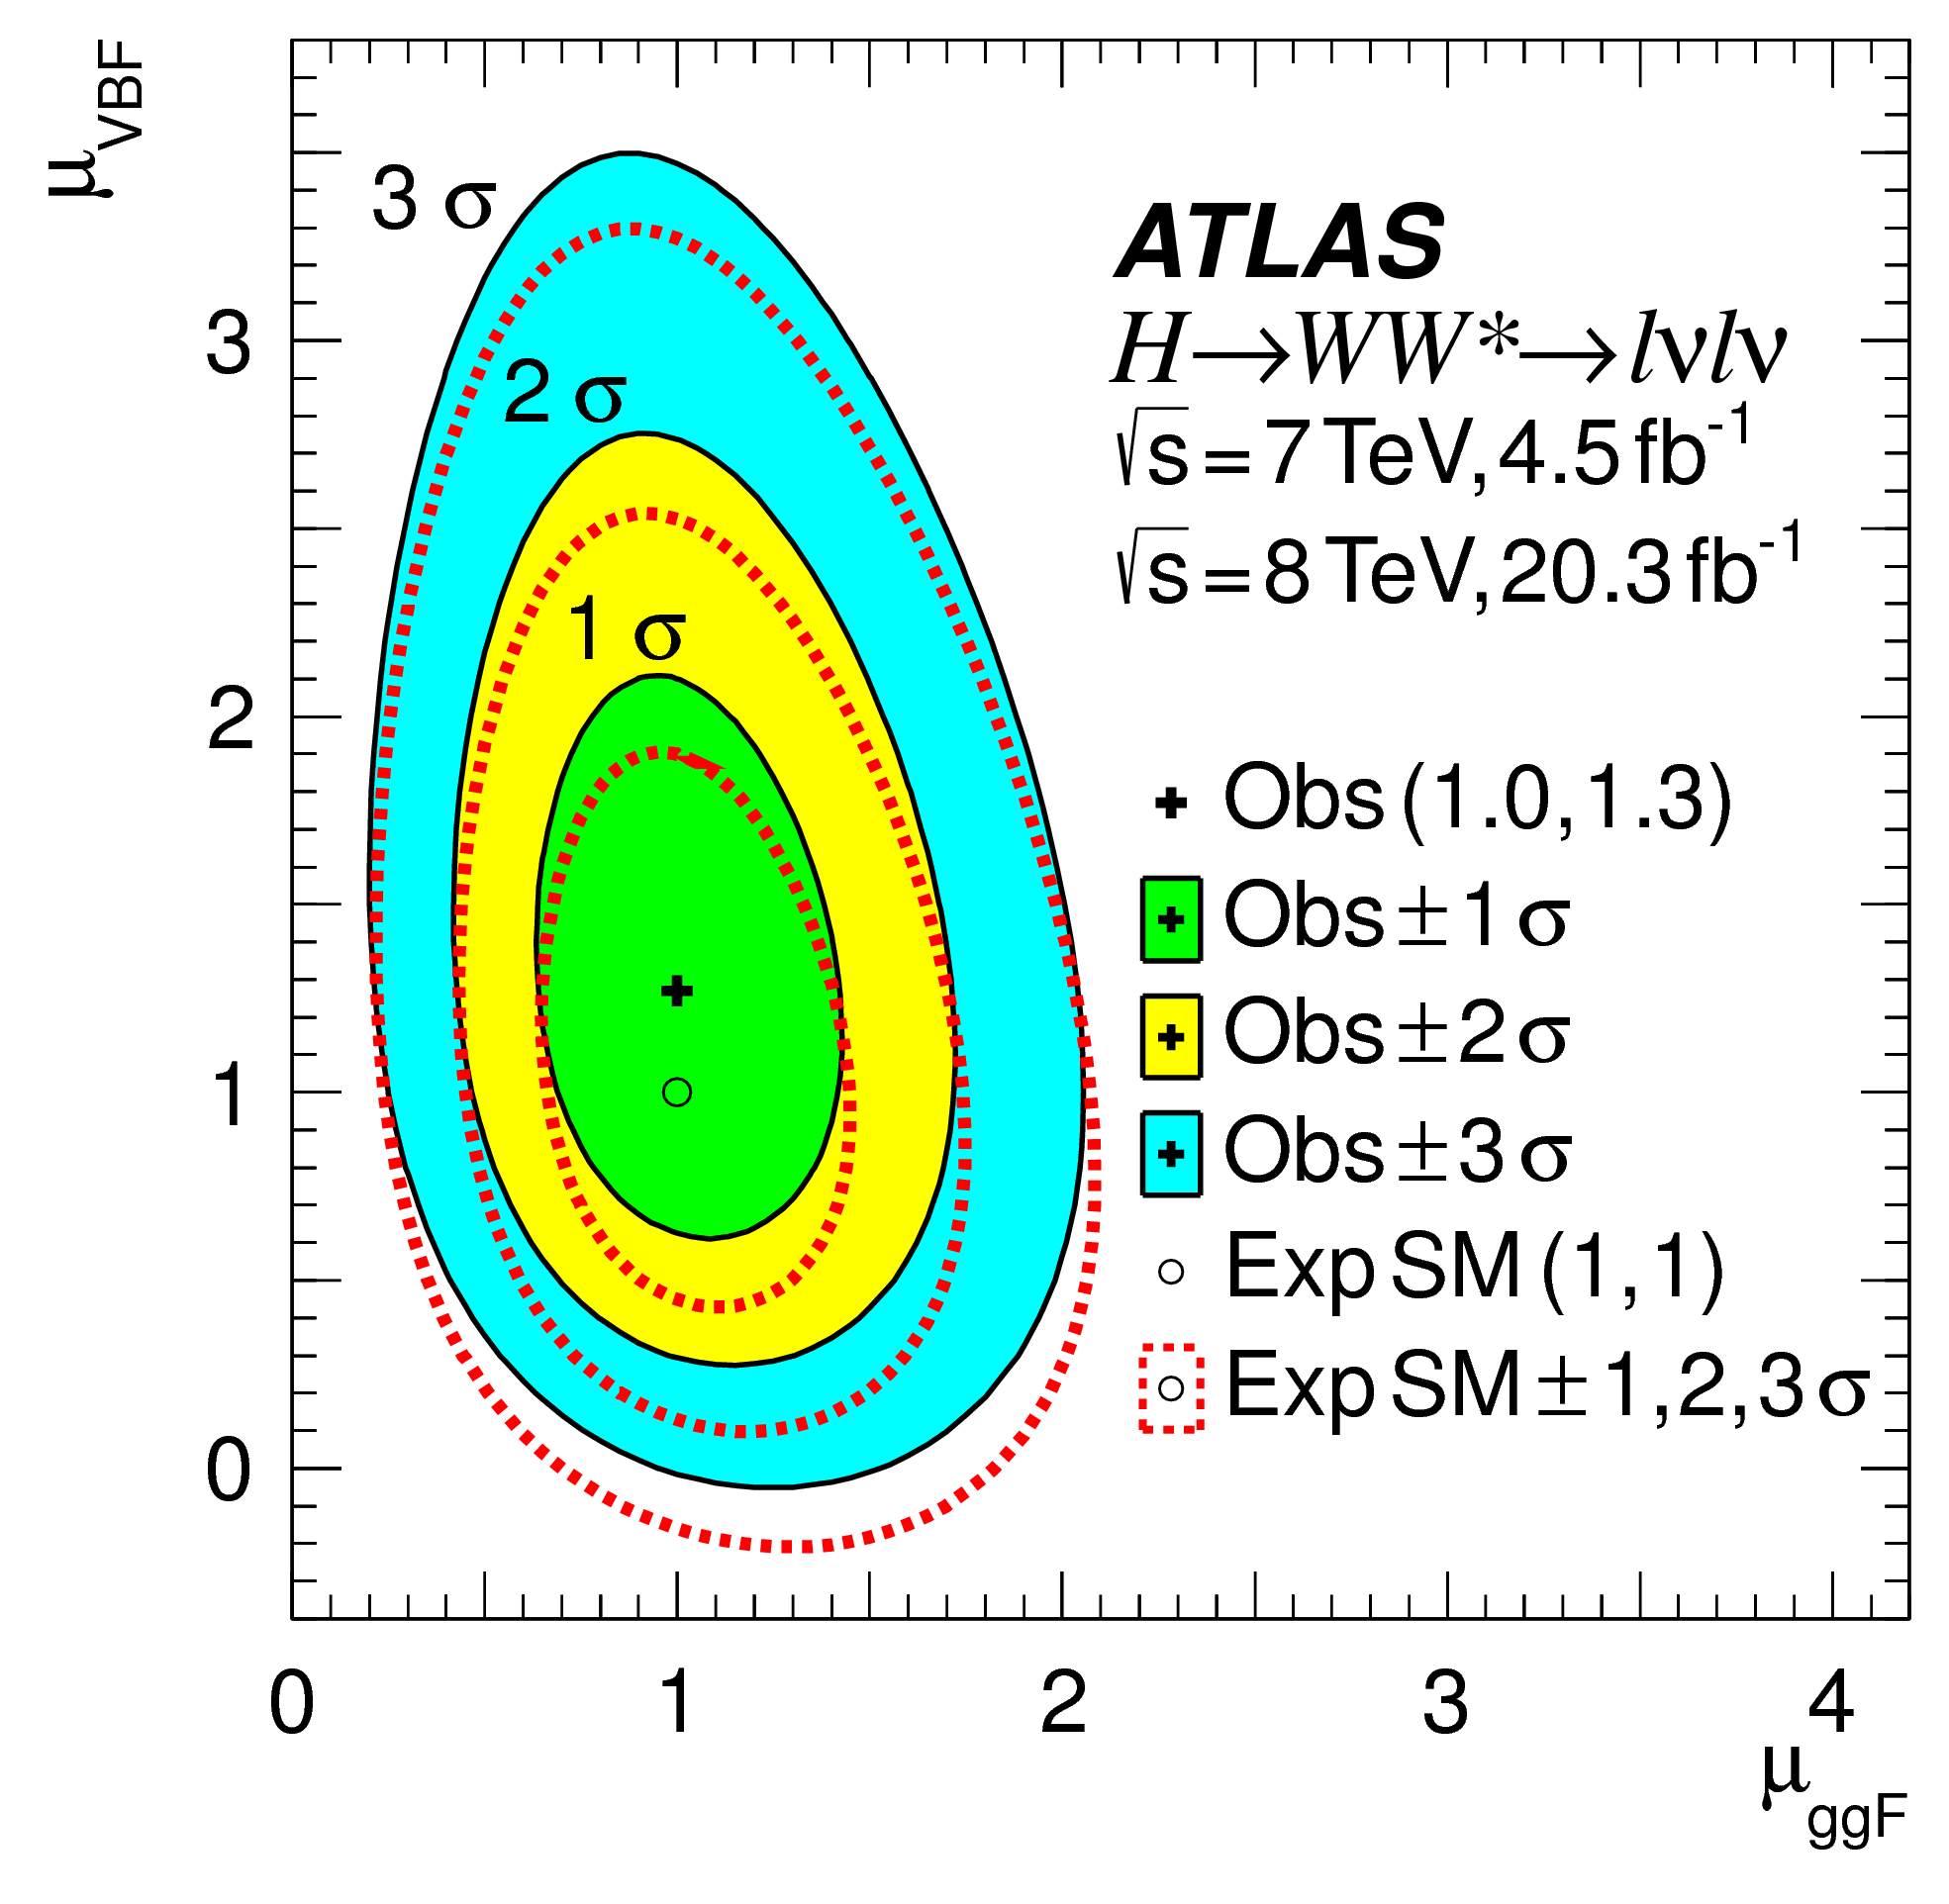
\includegraphics[width=0.7\textwidth]{figures/WW_muind}
  \caption{Likelihood scan as a function of $\mu_{\VBF} and \mu_{\ggF}$\cite{WW2015}.}
  \label{fig:mu_2d}
\end{figure}

\section{Measurement of Higgs couplings to vector bosons and fermions}





